\documentclass{article}
\usepackage{graphicx}
\usepackage[utf8]{inputenc}
\usepackage{amsmath, amssymb, latexsym}

\usepackage{pgfplots}
\usepackage{algorithm}
\usepackage[noend]{algpseudocode}
\usepackage{tikz}
\usepackage{nicefrac}
\pgfplotsset{every axis legend/.append style={
at={(0,0)},
anchor=north east}}
\usetikzlibrary{shapes,positioning,intersections,quotes}
\usetikzlibrary{arrows.meta,
                bending,
                intersections,
                quotes,
                shapes.geometric}
                
\definecolor{darkgreen}{rgb}{0.0, 0.6, 0.0}
\definecolor{darkred}{rgb}{0.7, 0.0, 0.0}
\makeatletter
\def\BState{\State\hskip-\ALG@thistlm}
\makeatother
\title{Week 7}
\begin{document}
  \pagenumbering{gobble}
  \maketitle
  \newpage
  \pagenumbering{arabic}

\section*{Overfitting with linear regression}
\begin{itemize}
\item We will use our house pricing example yet another time.
\item If we fit a linear function to the data, we have underfitting - also known as high bias.
\item If we fit a quadratic function, it will fit better than a straight line, but it will not pass through all of the points.
\item If we fit 4th order polynomial, the curve fit's through all five examples. This is overfitting - also known as high variance.
\end{itemize}

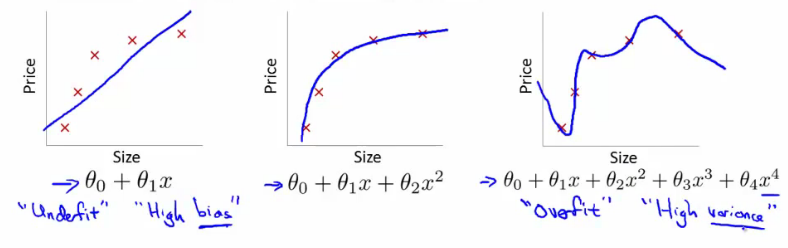
\includegraphics[width=\textwidth]{resources/overfitting_linear_regression}

\section*{Overfitting with linear regression}
\begin{itemize}
\item The same thing may happen with logistic regression.
\item Sigmoidal function is an underfit.
\item A high order polynomial, on the other hand, results in overfitting (high variance hypothesis).
\end{itemize}

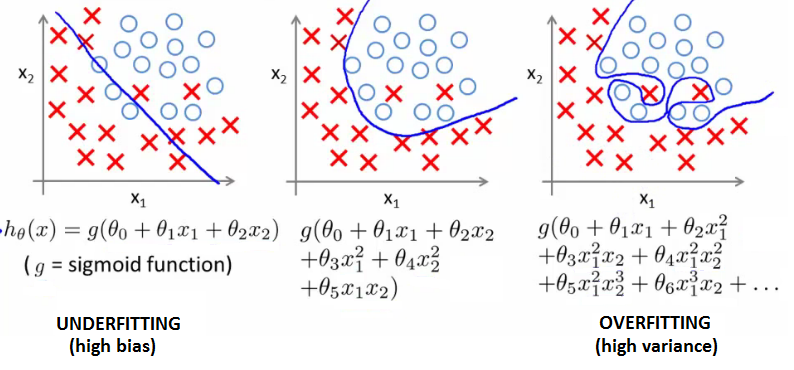
\includegraphics[width=\textwidth]{resources/overfitting_logistic_regression}


\section*{Cost function optimization for regularization}

Penalize and make some of the $\theta$ parameters really small.


$$min \frac{1}{2m} \sum_{i=1}^{m}(h_{\theta}(x^{(i)} + y^{(i)})^2 + 1000 \theta_3^2 +  1000 \theta_4^2$$

~\\
So we simply end up with $\theta_3$ and $\theta_4$ being near to zero (because of the huge constants) and we're basically left with a quadratic function.

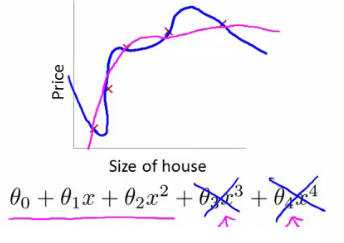
\includegraphics[width=0.5\textwidth]{resources/optimization_regularization}

~\\
Regularization\\
Small parameter values correlate to a simpler hypothesis (you effectively get rid of some of the terms). Overfitting is less likely with a simpler hypothesis.

$$J(\theta) = \frac{1}{2m} [ \sum_{i=1}^{m}(h_{\theta}(x^{(i)} + y^{(i)})^2 + \lambda \sum_{j=1}^{m} \theta_j^2] $$

~\\
$\lambda$ is the regularization parameter that controls a trade off between our two goals:

\begin{itemize}
\item Want to fit the training set well.
\item Want to keep parameters small.
\end{itemize}

Later in the course, we'll look at various automated methods for selecting $\lambda$.


\section*{Regularized linear regression}

\begin{algorithm}
\caption{Regularized linear regression}\label{euclid}
\begin{algorithmic}[1]
\Large
\While {not converged}
\State $\theta_j := \theta_j - \alpha [\frac{1}{m} \sum_{i=1}^{m}(h_{\theta}(x^{(i)} + y^{(i)})x_j^{(i)} + \frac{\lambda}{m} \theta_j]$
\State $(for\ j = 1, 2, 3, ..., n)$
\EndWhile
\end{algorithmic}
\end{algorithm}

\section*{Regularization with the normal equation}

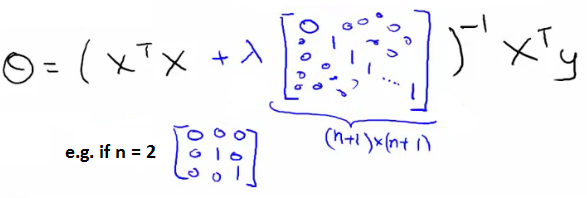
\includegraphics[width=0.8\textwidth]{resources/regularized_normal_equation}

\section*{Regularized logistic regression}

Logistic regression cost function is as follows:


$$J(\theta) = -[\frac{1}{m} \sum_{i=1}^{m} y^{(i)} log (h_{\theta}(x^{(i)} + (1- y^{(i)})log(1 - h_{\theta}(x^{(i)}))] +  \frac{\lambda}{2m} \sum_{j=1}^{m} \theta_j^2$$

\begin{algorithm}
\caption{Regularized logistic regression}\label{euclid}
\begin{algorithmic}[1]
\Large
\While {not converged}
\State $\theta_j := \theta_j - \alpha [\frac{1}{m} \sum_{i=1}^{m}(h_{\theta}(x^{(i)} + y^{(i)})x_j^{(i)} + \frac{\lambda}{m} \theta_j]$
\State $(for\ j = 1, 2, 3, ..., n)$
\EndWhile
\end{algorithmic}
\end{algorithm}

~\\
It appears to be the same as linear regression, except that the hypothesis is different.

\end{document}